%
% einleitung.tex -- Beispiel-File für die Einleitung
%
% (c) 2020 Prof Dr Andreas Müller, Hochschule Rapperswil
%
% !TEX root = ../../buch.tex
% !TEX encoding = UTF-8
%
\section{Einleitung\label{helmholtz:section:teil0}}
\kopfrechts{Teil 0}

\subsection{Mathematische Tools}

Hier werden kurz die Tools vorgestellt, welche für die Helmholtz-Zerlegung benötigt werden.

\subsubsection{Der Gradient eines Skalarfeldes $a$}
\begin{equation}
\nabla a(\mathbf{r}) = \frac{\partial a}{\partial x}\mathbf{e}_x + \frac{\partial a}{\partial y}\mathbf{e}_y + \frac{\partial a}{\partial z}\mathbf{e}_z
\end{equation}

Das Gradient (wie beschrieben in  \eqref{buch:kurvenintegral:differential:eqn:ricthungsableitung} ) wirkt auf ein Skalarfeld und liefert ein Vektorfeld, das in Richtung des steilsten Anstiegs von $a$ zeigt. Der Gradient an einem Punkt ergibt die Richtung maximaler Zunahme des Skalars an. Der Betrag entspricht der Steigung in der entsprechenden Richtung. \newline

% https://www.elektroniktutor.de/fachmathematik/nabla.html#:~:text=Richtung%20ihr%20Maximum,die%20Gr%C3%B6%C3%9Fe%20der%20Steigung%20an


\subsubsection{Die Divergenz eines Vektorfeldes $\mathbf{F}$}
\begin{equation}
\nabla \cdot \mathbf{F}(\mathbf{a}) = \frac{\partial F_x}{\partial x} + \frac{\partial F_y}{\partial y} + \frac{\partial F_z}{\partial z}
\end{equation}

Die Divergenzmiss für ein bestimmtes Vektorfeld $\mathbf{A}(\mathbf{r})$ die ?QUellendichte? , was bedeutet wie stark die Feldlinien auseinanderstreben (positive DIvergenz) oder zusammenlaufen (negative Divergenz). \newline

%https://www.elektroniktutor.de/fachmathematik/nabla.html#:~:text=Wird%20der%20Differenzialoperator%20Nabla%20skalar,Ist


\begin{figure}[h!]
	\centering
	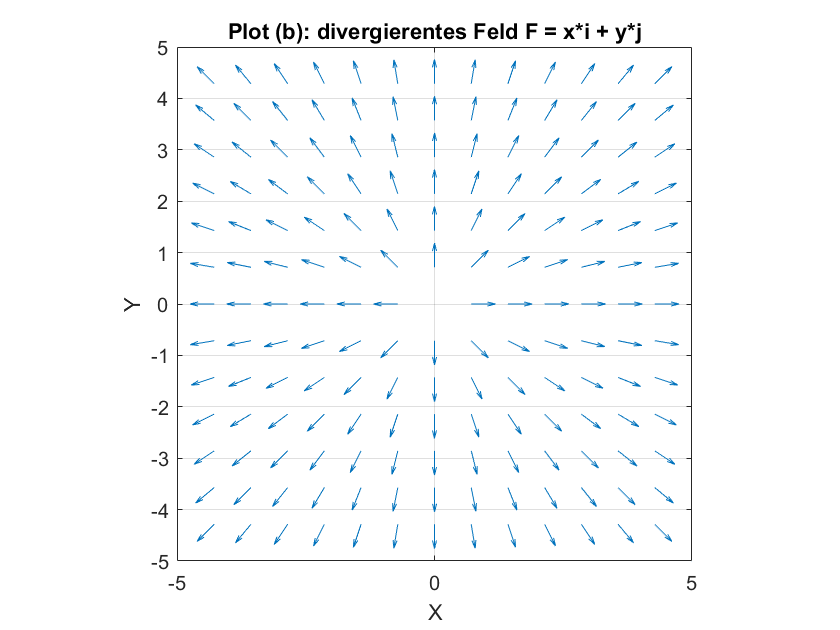
\includegraphics[scale=0.4]{papers/helmholtz/images/divergentes_Feld.png}
	\caption{Divergierendes Feld}
	\label{fig:DivergenzAlg}
\end{figure}




\subsubsection{Die Rotation eines Vektorfeldes}
\begin{equation}
\nabla \times \mathbf{A}(\mathbf{r}) = \begin{vmatrix}
	\mathbf{e}_x & \mathbf{e}_y & \mathbf{e}_z \\
	\frac{\partial}{\partial x} & \frac{\partial}{\partial y} & \frac{\partial}{\partial z}\\
	A_x & A_y & A_z
\end{vmatrix}
\end{equation}

\begin{figure}[h!]
	\centering
	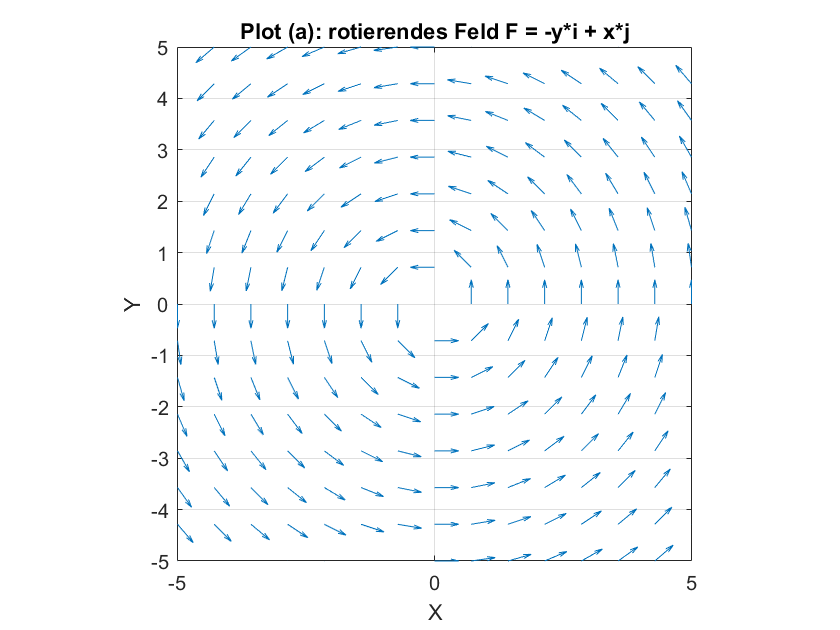
\includegraphics[scale=0.4]{papers/helmholtz/images/rotierendes_Feld.png}
	\caption{Rotation eines Vektorfeldes}
	\label{fig:LaplaceAlg}
\end{figure}

Die Rotation misst die Wirbeldichte eines Vektorfeldes $A$. Gleichtbedeutend mit wie stark sich die Feldlinien, um eine Achse drehen. Ein nichtverschwindendes $\nabla\times \mathbf{A}$ bedeutet, dass im Feld, Wirbel vorhanden sind: lokale Umlaufströmung. Insbesondere gibt $\nabla\times \mathbf{A}$ die Achsen-Ortientierung und Stärke eines solchen Wirbels an. Ist $\nabla\times \mathbf{A}=0$, so ist das Feld wirbelfrei (irrotational) \newline
% https://www.elektroniktutor.de/fachmathematik/nabla.html#:~:text=Kr%C3%A4ftefeld%2C%20so%20wird%20entlang%20eines,gilt%20das%20Feld%20als%20wirbelfrei



\subsubsection{Laplace-Operator eines Skalarfeldes}
\begin{equation}
\nabla^2 a(\mathbf{r}) = \frac{\partial^2 a}{\partial x^2} + \frac{\partial^2 a}{\partial y^2} + \frac{\partial^2 a}{\partial z^2}
\end{equation}

\begin{figure}[h!]
	\centering
	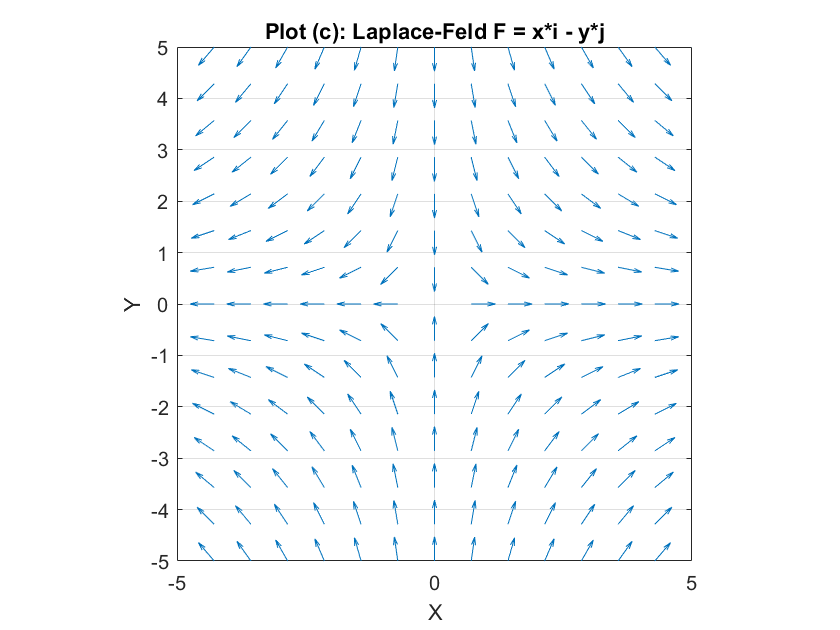
\includegraphics[scale=0.4]{papers/helmholtz/images/Laplace_Feld.png}
	\caption{Laplace eines Feldes}
	\label{fig:LaplaceAlg}
\end{figure}


\subsection{Physikalische Grundlage}

Um das Beispiel in der der Helmholtz-Zerlegung zu verstehen, bedarf es an Wissen aus der Akustik. Hierzu werden die 3 notwendigen physikalischen Grössen Schalldruck, Schallschnelle und Intensität erklärt. Vorzugsweise werden die Formeln in dem Freqeunezbereich (Fourier- Transfomierte) aufgeschrieben, da in vielen akustischen Aufgaben mit der komplexen Schreibweise gearbeitet wird.


\subsubsection{Schalldruck $p$}
\begin{itemize}
\item $P \: (\mathbf{r})$ die Amplitude des Drucks am Ort $r$ (reelle Grösse).
\item $\omega$ Kreisfrequenz.
\item $\phi \: (r)$ die Phase am Ort $r$ (reelle Grösse).
\end{itemize}

\begin{equation}
p(r,t) =  = P(r) \: e^{j( \omega t - \phi(r))} \qquad [\si{\pascal}]
\end{equation}

Frequenzbereich (Phasor-Darstellung) bei einer festen Frequenz $\omega$:

\begin{equation}
p(r) = P(r) \: e^{j \phi (r)}
\label{helmholtz:PhasorSchalldruck}
\end{equation}

\subsubsection{Schallschnelle  $u$}
Die Schallschnelle $u$ (Teilchengeschwindigkeit) wird aus dem Druckgradienten $\nabla p$ abgeleitet. Für die linearisierte Form $ \rho \frac{\partial u}{\partial t} = - \nabla p$ von harmonischen Felder $u(r,t)$  ergibt sich:

\begin{equation}
u(r,t) = \frac{1}{\omega \rho} \nabla \: p(r,t) = \frac{1}{\omega \rho} \bigg[ P(r) \nabla \Phi(r) + j\nabla P(r)  \bigg] \: e^{j[\omega t -\Phi(r)]} \qquad [\si{\metre / \second}]
\end{equation}

\begin{itemize}
\item $\nabla \phi \: (r)$ der Gradient der Phase (zeigt in Richtung der schnellsten Phasenänderung, senkrecht zur Wellenfront).
\item $\nabla P \:(r)$ der Gradient der Druckamplitude (zeigt in Richtung der schnellsten Amplitudenänderung).
\item $\rho$: Dichte des Materials
\end{itemize}

ergibt als Phasor bei einer fixen Frequenz $\omega$:

\begin{equation}
u(r) = \underbrace{\frac{1}{\omega p} \: \bigg[ P(r) \: \nabla \phi(r) + j - \nabla P(r) \bigg] \: e^{j\phi (r)}}_{}
\label{helmholtz:PhasorSchallschnelle}
\end{equation}

\subsubsection{Instantane Intensität $\vec{I} (r, t$)}

Die instantane Intensität $\vec{I}$ oder auch Momentan-Intensität, beschreibt die Energie pro Zeiteinheit durch eine senkrechte zur Ausbreitungsrichtung stehende Einheitsfläche und ist somit eine vektorielle Grösse. Sie ist als punktweies Produkt des momentanen Schalldrucks und der momentanen Schallschnelle definiert.

Die pseudo physikalische definition (um ein Bild der physikalischen Grösse zu erhalten) lautet:

\begin{equation}
\textit{Intensität} = \textit{Druck} \cdot \textit{Schnelle}=\frac{\textit{Kraft}}{\textit{Fläche}} \cdot \frac{\textit{Weg}}{\textit{Zeit}} = \frac{\textit{Energie}}{\textit{Fläche}\cdot \textit{Zeit}} = \frac{\textit{Leistung}}{\textit{Fläche}}.
\label{helmholtz:equationIntensitaetPseudoDef}
\end{equation}

und die korrekte physikalische Definition ist:

\begin{equation}
\mathbf{|\vec{I}|} \:(r ,t)  =  \operatorname{Re}{p(r, t)} \cdot \operatorname{Re}{u(r, t)} \qquad [\si{\W / \square\metre}]
\label{helmholtz:equationIntensitaetMomentan}
\end{equation}


\subsubsection{Komplexe Intensität ($I_c$)}

Um die Helmholtz-Zerlegung anhand der Schallintensität aufzuzeigen, wird die Komplexe Intensität benötigt. Ist wie folgt definiert:

\begin{equation}
\mathbf{\vec{I}}_c (r)  = \frac{1}{2} \:  p(r) \: u^{*}(r) 
\label{helmholtz:equationIntensitaetKomplex}
\end{equation}

Die Komplexe Intensität enthält 2 wichtige Grössen nähmlich die aktive Intensität $\mathbf{I}(r)$ und die reaktive Intensität $\mathbf{Q}(r)$. 

\begin{equation}
	\mathbf{I}_c ~(\mathbf{r}) = \underbrace{\mathbf{I}~(\mathbf{r})}_{\textit{aktive Intensität}} + \underbrace{j\,\mathbf{Q}~(\mathbf{r})}_{\textit{reaktive~Intensität}}
\label{helmholtz:equationIntensitaetKomplex_2}
\end{equation}	

\begin{itemize}
\item Die aktive Intensität $\mathbf{I}(r)$ (Realteil) ist die zeitgemittelte Netto-Energiefluss pro Fläche an dem Ort $r$.
\begin{equation}
	\mathbf{I}~(\mathbf{r}) = \frac{1}{T}\int_0^T \mathbf{I}_i(\mathbf{r},t)\,~\mathrm{d}t = \frac{1}{2}\Re\left\{P(\mathbf{r})~\mathbf{U}^*(\mathbf{r})\right\}
	\end{equation}
\begin{equation}
	\nabla \cdot \mathbf{I} = 0 \qquad \text{keine Quellen oder Senken}
\end{equation}
\begin{equation}
	\nabla \times \mathbf{I} = \frac{k}{c} \frac{\mathbf{I} \times \mathbf{Q}}{V}
\end{equation}
\item Die reaktive Intensität $\mathbf{Q}(r)$ (Imaginärteil) beschreibt die zeitlichgemittelte Dichte der nicht-propagierenden, oszilierenden Energie. 
\begin{equation}
	\mathbf{Q}(\mathbf{r}) = \frac{1}{2}\Im\left\{P(\mathbf{r})~\mathbf{U}^*(\mathbf{r})\right\}
	\label{helmholtz:equationReaktiveIntensitaet}
	\end{equation}
\begin{equation}
	\nabla \times \mathbf{Q} = 0 \qquad \text{wirbelfrei}
\end{equation}
\begin{equation}
	\nabla \cdot \mathbf{Q} = -2 \omega [T-V]
\end{equation}
\end{itemize}




